\documentclass[22pt]{article} 
\usepackage{geometry} 
\usepackage{float} 
\usepackage{graphicx}
\usepackage{caption}
\usepackage{subfigure}
\usepackage{amsmath}
\usepackage{array}
\usepackage{amsfonts,amssymb} %空心字符
\usepackage{listings}
\usepackage[framed,autolinebreaks,useliterate]{mcode}%matlab
\geometry{left=2.0cm,right=2.0cm,top=0.5cm,bottom=0.5cm}
	\author{Mengfan Wang} 
	\title{Optimization Techniques Homework 3} 
\begin{document}
	\maketitle 
	\paragraph{1}
	Because $A$ is a real symmetric matrix, $A$ can be decomposed as $A = Q\Lambda Q^T$,while $Q$ is orthogonal. Then we have:
	\begin{equation}
		Q^TAQ = Q^TQ\Lambda Q^TQ = \Lambda
	\end{equation}
	If $Q$ is represented as column vectors $[q_1\ q_2\ q_3\ \dots q_n]$:
	\begin{equation}
		\left[ \begin{array}{c} q_1^T \\ q_2^T \\ \vdots\\ q_n^T \end{array} \right] A [q_1\ q_2\ \dots q_n] = \Lambda
	\end{equation}
	So, 
	\begin{equation}
		q_i^TAq_j = \begin{cases}
			\lambda_i& i=j\\
			0& i\not=j
			\end{cases}
	\end{equation}
	And $q_1$ to $q_j$ are linearly independent. For any $x\in \mathbb{R}^n$, $x$ can be represented as $x = \sum\limits_{i=1}^na_iq_i$. Because $x^Tx = 1$:
	\begin{align}
		(\sum\limits_{i=1}^na_iq_i^T)(\sum\limits_{j=1}^na_jq_j) & = 1\\
		\sum\limits_{i=1}^na_i(\sum\limits_{j=1}^na_jq_i^Tq_j) & = 1\\
		\sum\limits_{i=1}^na_i^2 & = 1
	\end{align}
	And then:
	\begin{align}
		x^TAx & = (\sum\limits_{i=1}^na_iq_i^T)A(\sum\limits_{j=1}^na_jq_j)\\
		& = \sum\limits_{i=1}^na_i(\sum\limits_{j=1}^na_jq_i^TAq_j)\\
		& = \sum\limits_{i=1}^na_i(a_i \lambda_i)\\
		& = \sum\limits_{i=1}^na_i^2 \lambda_i
	\end{align}
	So, $x^TAx = \sum\limits_{i=1}^na_i^2 \lambda_i \leq \sum\limits_{i=1}^na_i^2 \lambda_1  = \lambda_1$, and $\sum\limits_{i=1}^na_i^2 \lambda_i \geq \sum\limits_{i=1}^na_i^2 \lambda_n = \lambda_n$, while $\lambda_1$ is the biggest eigenvalue and $\lambda_n$ is the smallest one. In conclusion, $\lambda_1\geq x^TAx \geq \lambda_n$.

	\paragraph{2} Define $X = [X_1,\dots,X_N]$, and $S = \sum\limits_{k=1}^{N}X_kX_k^T = XX^T$. Because $m$ is assumed  to $0$, $a_k = e^TX_k = X_k^Te$. So the objective function equals to:
	\begin{align}
		& min_e \sum\limits_{k=1}^{N} (X_k - ea_k)^T(X_k - ea_k)\\
		= & min_e \sum\limits_{k=1}^{N} (\|X_k\|^2 - 2a_ke^TX_k + a_k^2\|e\|^2)\\
		= &  min_e \sum\limits_{k=1}^{N} (-a_k^2 +\|X_k\|^2 ) \\
		= &   min_e - \sum\limits_{k=1}^{N} e^TX_kX_k^Te +  \sum\limits_{k=1}^{N} \|X_k\|^2\\
		= &   min_e - e^T (\sum\limits_{k=1}^{N} X_kX_k^T)e +  \sum\limits_{k=1}^{N} \|X_k\|^2\\
		= &   min_e -  e^TSe +  \sum\limits_{k=1}^{N} \|X_k\|^2 \label{1}
	\end{align}
	Set $\lambda$ is the Lagrange multiplier and the Lagrangian function is:
	\begin{align}
		L(\lambda,e) = -  e^TSe +  \sum\limits_{k=1}^{N} \|X_k\|^2 + \lambda (e^Te - 1)
	\end{align}
	The original objective function is minimum only when the derivative of Lagrangian function is 0:
	\begin{align}
		\frac{\partial L}{\partial e}  = -2Se + 2 \lambda e & = 0\\
		Se & = \lambda e \label{2}
	\end{align}
	As a result, $\lambda$ is an eigenvalue of $S$ and $e$ is the corresponding eigenvector. Combine Eq.\ref{1} and Eq.\ref{2}, the objective function is:
	\begin{align}
		 & min_e -  e^T 	\lambda e +  \sum\limits_{k=1}^{N} \|X_k\|^2 \\
		  = & min_e - \lambda +  \sum\limits_{k=1}^{N} \|X_k\|^2 
	\end{align}
	To get the minimum, $\lambda$ should be the largest eigenvalue of $S$. So, $e = v_1$ and $a_k = e^TX_k = v_1^TX_k$.

	\paragraph{3}Set $\lambda$ is the Lagrange multiplier and the Lagrangian function is:
	\begin{align}
		L(\lambda,\gamma,w) & = tr[(XX^T-	\gamma ww^T)^2] + \lambda (ww^T-1)\\
		& = tr[XX^TXX^T - 2 \gamma XX^Tww^T+ \gamma^2 ww^T] + \lambda (ww^T-1) 
	\end{align}
	The original objective function is minimum only when the derivative of Lagrangian function is 0:
	\begin{align}
		\frac{\partial L}{\partial \gamma} = & -2 XX^Tww^T + 2\gamma ww^T = 0\\
		& \gamma ww^T = XX^Tww^T\label{3}
	\end{align}
	\begin{align}
		\frac{\partial L}{\partial w} = & -4 \gamma XX^Tw + 2 \gamma^2 w + 2\lambda w = 0\\
		& XX^Tw = \frac{\gamma^2+\lambda}{2	\gamma}w  \label{4}
	\end{align}
	Or $\gamma$ may be zero. Combine Eq.\ref{3} and Eq.\ref{4}, we have:
	\begin{align}
		\gamma ww^T & = \frac{\gamma^2+\lambda}{2	\gamma}ww^T\\
		\gamma^2 &= \lambda
	\end{align}
	\begin{align}
		XX^Tw = \frac{\gamma^2+\lambda}{2\gamma}w = \gamma w
	\end{align}
	So, $\gamma$ is an eigenvalue of $XX^T$ and $w$ is the corresponding eigenvector, or $\gamma = 0$. Now proving $\gamma$ must be the largest eigenvalue. Because $XX^T$ is symmetric, it can be decomposed as $XX^T = Q \Lambda Q^T$, and the original objective function is:
	\begin{align}
		& \min_{\gamma,w} tr[(XX^T-	\gamma ww^T)^2]\\
		= & \min_{\gamma,w} tr[QQ^T(Q \Lambda Q^T-	\gamma ww^T)^2]\\
		= & \min_{\gamma,w} tr[(\Lambda -	\gamma Q^T ww^TQ)^2]
	\end{align}
	The columns of $Q$ are eigenvectors of $XX^T$. Suppose $Q = [w_1\ w_2 \ \dots \ w_n]$, and $w = w_k$ is one column of $Q$:
		\begin{align}
			Q^T ww^TQ & = \left[ \begin{array}{c} w_1^T\\ w_2^T\\ \vdots\\ w_n^T \end{array} \right]w_kw_k^T[w_1\ w_2 \ \dots \ w_n]\\
			& = \left[ \begin{array}{c} 0\\ 0\\ \vdots\\ 1\\ \vdots\\ 0 \end{array} \right]*[0\ 0\ \dots 1\ \dots 0]\\
			& = \delta_{kk},
		\end{align}
	while $\delta_{kk}$ means a matrix has $1$ at the position $(k,k)$ and all other entries are $0$. And the objective function equals to:
	\begin{align}
		& \min_{\gamma,w} tr[(\Lambda -	\gamma Q^T ww^TQ)^2]\\
		= & \min_{\gamma,w} tr[(\Lambda -	\gamma \delta_{kk})^2]\\
		= & \min_{\gamma,w} tr(\Lambda^2) - \gamma^2
	\end{align}
	 To get the minimum, $\gamma$ should be the largest eigenvalue of $XX^T$. 

	In conclusion, the solution is that $\gamma$ is the largest eigenvalue of $XX^T$ and $w$ is the corresponding eigenvector.

	\paragraph{4} The PCA algorithm is based on SVD. Suppose $X = U \Sigma V^T$, and $XX^T = U \Sigma V^T V \Sigma U^T= U \Sigma^2 U^T$. So the columns of $U$ is the eigenvectors of $XX^T$, which is sorted as the size of corresponding eigenvalues.

	Source code:
	\begin{lstlisting}
clc;clear;close all;

data = xlsread('datamatrix.csv');
data = data(:,2:2794);
data = PCA(data,2);
plot(data(1,:),data(2,:),'r.');

function data_PCA = PCA(data,dimension)
    %This function is used to implement PCA algorithm.
    %Input:  data-------- Each column is a data point. All data points
    %                     should have the same dimension of features.
    %        dimension--- The dimension data will be reduced to.
    %Output: data_PCA---- The new data after transformation. Each column
    %                     is a data point.
    
    data = (data-mean(data,2))./sqrt(var(data,[],2)); %normalization
    [U,S,V] = svd(data);
    data_PCA = U(:,1:dimension)'*data;
end
	\end{lstlisting}

	The result reduced to 2 dimensional space is visualized in Figure.1.

	\begin{figure}[H]
				\centering
				\subfigure{
					\begin{minipage}{14cm}
					\centering 
					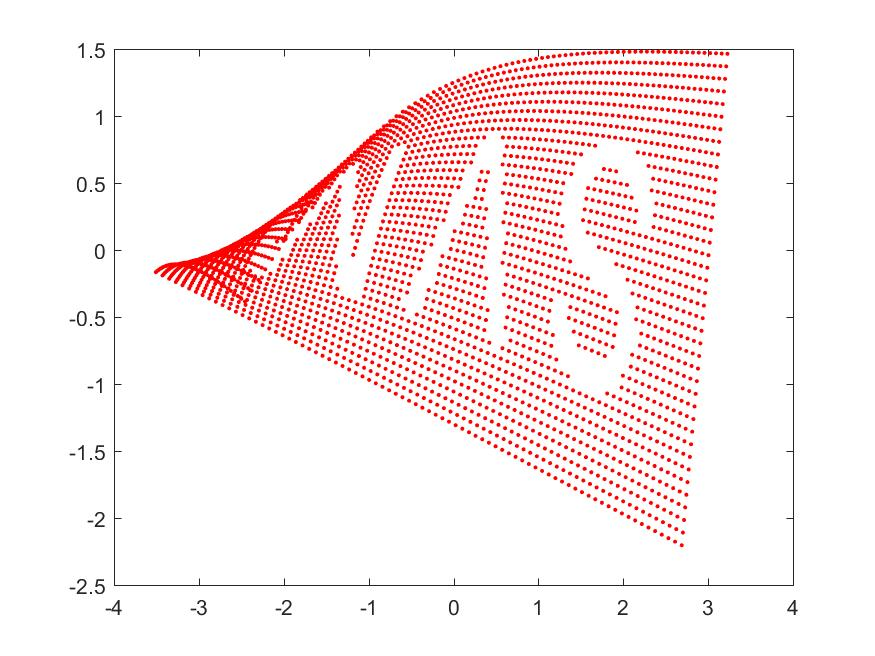
\includegraphics[height=7cm]{q4.jpg}
					\end{minipage}
				}
				\caption{The visual result}
			\end{figure}

	\paragraph{5} LDA is not applicable to the data, because LDA is a supervised learning algorithm but the dataset doesn't contain any labels. If we want to use LDA, the dataset has to be divided into one or more classes. However, to make sure the result won't change by the dividing method, only two ways are there: Classify all data samples into the same class or classify each sample a class.

	For the first case, because there are only one class, $\mu_j = \mu$, and $S_B = \sum\limits_{j=1}^{k}N_j(\mu_j- \mu)(\mu_j- \mu)^T = (\mu- \mu)(\mu- \mu)^T = 0 $, $S_W^{-1}S_B=0$.  Therefore, the eigenvalues and eigenvectors of $S_W^{-1}S_B$ can only be zero, and we can't find a transformation to reduce the dimension.

	For the second case, because each sample has a class, $x_j = \mu_j$. $S_W = \sum\limits_{j=1}^{k} \sum\limits_{x\in X_j}(x- \mu_j)(x- \mu_j)^T = \sum\limits_{j=1}^{k}(x_j-x_j)(x_j-x_j)^T=0 $. $S_W^{-1}S_B$ is 0, too. 

	In conclusion, LDA is not applicable to the data no matter how to divide the dataset.
	
	\paragraph{6}
	The source code is based on the algorithm from LLE homepage. It's worth to mention that because the number of neighbors is set as more than the intrinsic dimension, the local covariance matrix $Z=(x_i-x_j)^T(x_i-x_j)$ isn't full rank and can't calculate $W$. In this case, it should be regularized by setting $Z = Z+eI$, while $e = 10^{-3}tr(C)$.

	Source code:
	\begin{lstlisting}
clc;clear;close all;

data = xlsread('datamatrix.csv');
X = data(:,2:2794);
d = 2;
for ii = 1:4
    if ii == 1
        K = 5;
    elseif ii == 2
        K = 10;
    elseif ii == 3
        K = 20;
    elseif ii == 4
        K = 100;
    end
Y = LLE(X,K,d);
figure(ii),plot(Y(1,:),Y(2,:),'r.');
end

function [Y] = LLE(X,K,d)
    %This function is used to implemeant LLE algorithm.
    %Input:  X----------- Each column is a data point. All data points
    %                     should have the same dimension of features.
    %        K----------- The number of neighbors.
    %        d----------- The dimension data will be reduced to.
    %Output: Y----------- The new data after transformation. Each column
    %                     is a data point.
    [D,N] = size(X);

    distance = dist(X',X);
    
    % find neighbors
    [sorted,index] = sort(distance);
    neighbor = index(2:(1+K),:);
    
    % If K>D, the local covariance will not be full rank
    if K>D
      tol=0.001; 
    else
      tol=0;
    end
    
    %Calculate W
    W = zeros(K,N);
    for ii=1:N
       x_ij = X(:,neighbor(:,ii))-repmat(X(:,ii),1,K);
       Z = x_ij'*x_ij;                                     
       Z = Z + eye(K,K)*tol*trace(Z);                   
       W(:,ii) = Z\ones(K,1);                        
       W(:,ii) = W(:,ii)/sum(W(:,ii));                
    end

    %Calculte M
    M = sparse(1:N,1:N,ones(1,N),N,N); 
    for ii=1:N
       w = W(:,ii);
       jj = neighbor(:,ii);
       M(ii,jj) = M(ii,jj) - w';
       M(jj,ii) = M(jj,ii) - w;
       M(jj,jj) = M(jj,jj) + w*w';
    end
    
    %Use eigen decomposition to get the new data
    [Y,values] = eigs(M,d+1,0);
    Y = Y(:,1:d)'; 

end
	\end{lstlisting}

	Figure 2 shows the results. It can be seen that there are 3 capital English letters ``SVM'' embedded in the data. In conclusion, the setting neighbors equaling to 100 is best. The reason is the relationship between a data point and its neighbors is considered to be linear and will not change after transformation. If the number of neighbors is too small, the algorithm will focus on a small local area. The continuous manifold can falsely be divided into disjoint sub-manifolds, and the
	mapping does not reflect so much global properties(Figure 2(a) and 2(b)). 
	\begin{figure}[H]
				\centering
				\subfigure{
					\begin{minipage}{7cm}{(a)5 neighbors}
					\centering 
					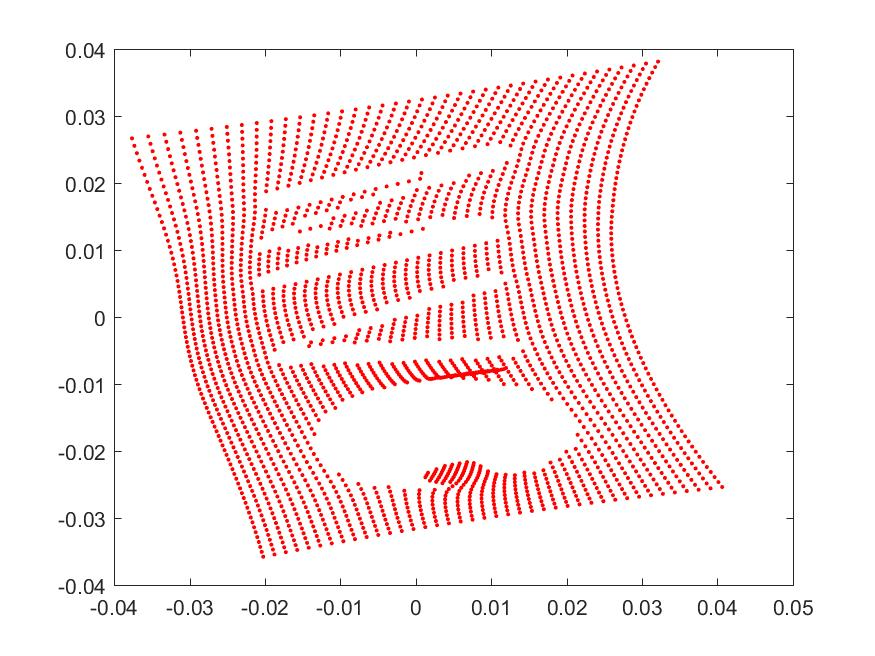
\includegraphics[height=5cm]{5.jpg}
					\end{minipage}
				}
				\subfigure{
					\begin{minipage}{7cm}{(b)10 neighbors}
					\centering 
					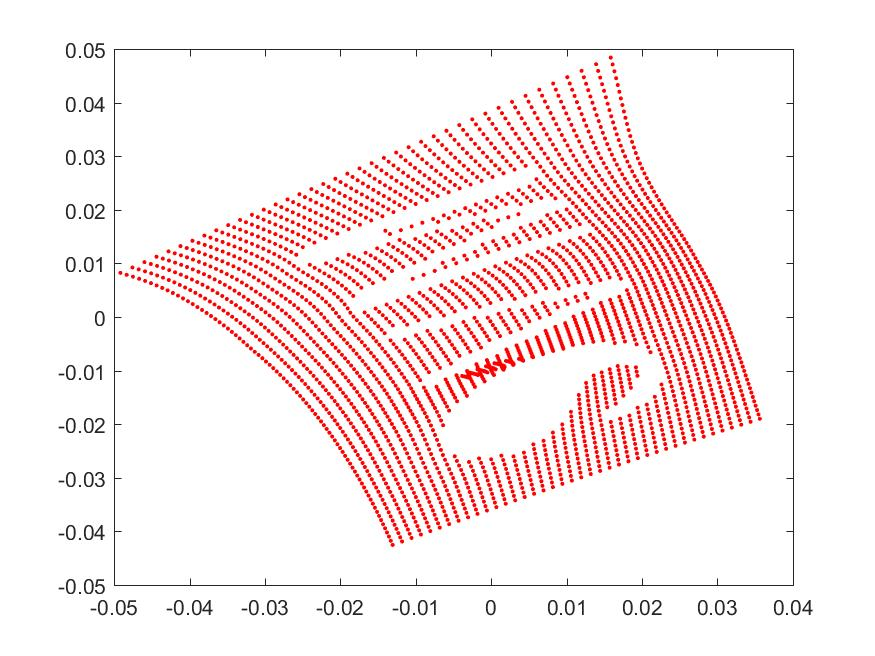
\includegraphics[height=5cm]{10.jpg}
					\end{minipage}
				}
				\subfigure{
					\begin{minipage}{7cm}{(c)20 neighbors}
					\centering 
					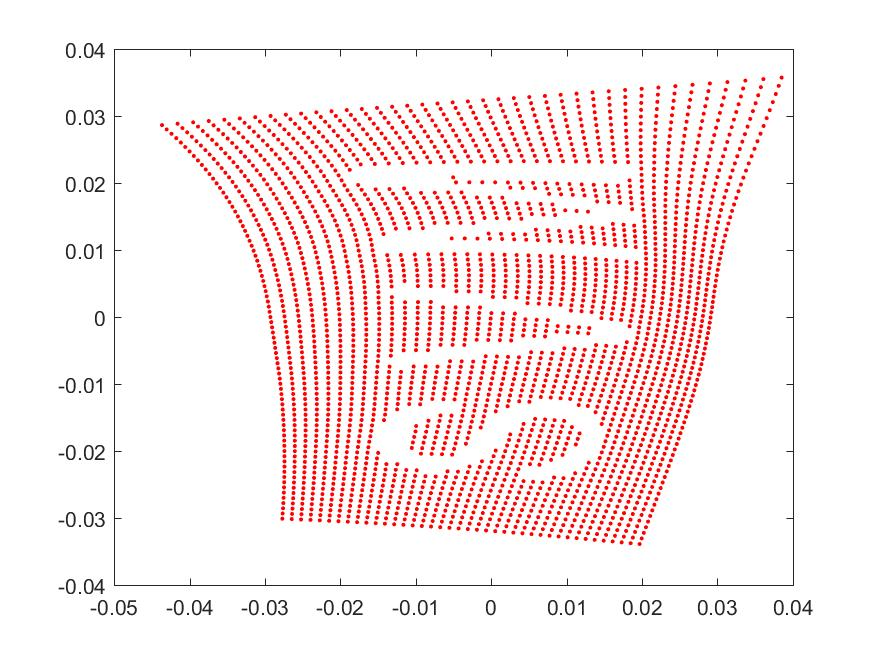
\includegraphics[height=5cm]{20.jpg}
					\end{minipage}
				}
				\subfigure{
					\begin{minipage}{7cm}{(d)100 neighbors}
					\centering 
					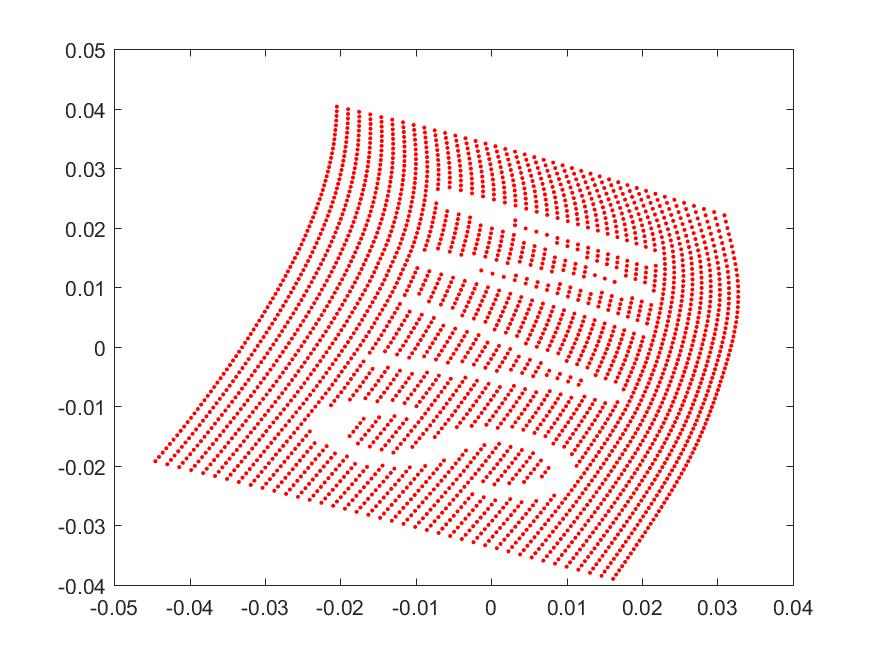
\includegraphics[height=5cm]{100.jpg}
					\end{minipage}
				}
				\caption{Results of different neighbors.}
			\end{figure}

	On the other hand, if the number of neighbors is too large, the algorithm can't focus on a local area but take the high dimension properties into account, which will causes smoothing or elimination of small-scale structures in the manifold. The mapping loses its nonlinear character, and degenerate to PCA. Figure 3 shows the result with neighbors equaling to 1000, which is one third of the whole dataset. The result is similar to Question 5's result.
	\begin{figure}[H]
				\centering
				\subfigure{
					\begin{minipage}{14cm}
					\centering 
					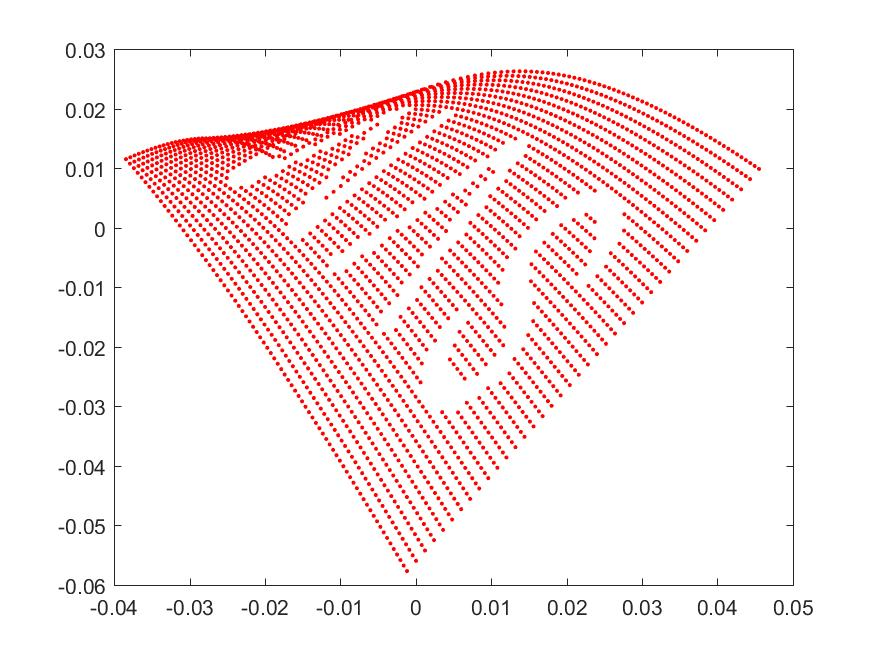
\includegraphics[height=7cm]{1000.jpg}
					\end{minipage}
				}
				\caption{Results when neighbors = 1000.}
			\end{figure}

\end{document}

